
\vspace{-.1in}
\section{Experiments}\label{sec:experiments}
In this section, we conduct experiments on the attacks on contextual bandit problems with simulated data and two real-word datasets: MovieLens25M \cite{harper2015movielens} and Jester \cite{goldberg2001eigentaste}. The synthetic dataset and the data preprocessing step are presented in App.~\ref{app:experiments_setup}.
\vspace{-0.05in}
\subsection{Attacks on Rewards}
\vspace{-0.02in}
We study the impact of the reward attack for $4$ contextual algorithms: \linucb, \lints, \epsgreedy and \expfour. As parameters, \changebr{we use $L=1$ for the maximal norm of the contexts}, $\delta = 0.01$, $\upsilon = \sigma\sqrt{d\ln(t/\delta))/2}$, $\varepsilon_{t} = 1/\sqrt{t}$ at each time step $t$ and $\lambda = 0.1$. \changee{We choose only a \textit{unique target arm} $a^{\dagger}$.} For \expfour, we use $N = 10$ experts with $N-2$ experts returning a random arm at each time, one expert choosing arm $a^{\dagger}$ every time and one expert returning the optimal arm for every context. With this set of experts the regret of bandits with expert advice is the same as in the contextual case. To test the performance of each algorithm, we generate $40$ random contextual bandit problems and run each algorithm for $T = 10^{6}$ steps on each. We report the average cost and regret for each of the $40$ problems.  
% \begin{figure}[t]
% \centering
% % \includegraphics[width=0.45\textwidth]{images/rewards_attacks_simulations/gen_synth_regret.pdf}
% \includegraphics[width=.4\textwidth]{images/rewards_attacks_simulations/gen_synth_cost.pdf}
% \caption{Total cost of attacks for synthetic data with $\gamma = 0.22$.}
% \label{fig:synthetic_reward_stochastic}
% \end{figure}
Figure \ref{fig:costs_plot} (Top) shows the attacked algorithms using the attacked reward $\wt{r}^{1}$ (reported as ``stationary CACE'') and the rewards $\wt{r}^{2}$ (reported as CACE).


These experiments show that, even though the reward process is non-stationary,  usual stochastic algorithms like \linucb can still adapt to it and pull the optimal arm for this reward process (which is arm $a^{\dagger}$). The true regret of the attacked algorithms is linear as $a^{\dagger}$ is not optimal for all contexts. %At $T = 10^{6}$.\todol{There misses sth here?}
In the synthetic case, for the algorithms attacked with the rewards $\wt{r}^{2}$, over 1M iterations and $\gamma = 0.22$, the target arm is drawn more than $99.4\%$ of the time on average for every algorithm and more than $97.8\%$ of the time for the stationary attack $\wt{r}^1$ (see Table~\ref{table:number_of_draws} in App.~\ref{app:additional_fig_rwds}). The dataset-based environments (see Figure~\ref{fig:costs_plot} (Left)) exhibit the same behavior: the target arm is pulled more than $94.0\%$ of the time on average for all our attacks on Jester and MovieLens and more than $77.0\%$ of the time in the worst case (for \lints attacked with the stationary rewards) (see Table~\ref{table:number_of_draws}).
% \begin{figure}[h]
% \centering
% \includegraphics[width=0.4\textwidth]{images/rewards_attacks_jester/gen_jester_cost.pdf}
% \includegraphics[width=.4\textwidth]{images/rewards_attacks_movielens/gen_movielens_cost.pdf}
% \caption{Total cost of attacks on Jester (Top) and MovieLens (Bottom) with $\gamma = 0.5$.}
% \label{fig:dataset_reward_attacks}
% \end{figure}
% \begin{figure}[t]
% \centering
% \begin{tabular}{c c}
% Jester \vspace{-0.3cm} & MovieLens\\
% \includegraphics[width=.46\columnwidth]{images/costs_attacks_rewards_no_legend/gen_jester_cost.pdf}& 
% \includegraphics[width=.45\columnwidth]{images/costs_attacks_rewards_no_legend/gen_movielens_cost.pdf}\\
%  & Synthetic\\
% \includegraphics[width=.43\columnwidth]{images/costs_attacks_rewards_no_legend/legend_rewards_attacks.pdf}
% &
% 	\includegraphics[width=0.49\columnwidth]{images/costs_attacks_rewards_no_legend/gen_synth_cost.pdf}
% \end{tabular}%\\
% %	~\vspace*{-0.4cm}~\\
% \caption{Total cost of the attacks on the rewards on the synthetic and dataset-based environments with $\gamma =0.5$ for Jester and MovieLens and $\gamma=0.22$ for the synthetic dataset.\vspace{-0.8cm}}%. The cumulative cost of the attacks is sublinear and most attacks occur during the first few iterations.}
% \label{fig:costs_reward_attacks}
% \end{figure}

%\todol{Confidence sets on MovieLense?} they seem to be there, just very small
\vspace{-0.05in}
\subsection{Attacks on Contexts}\label{subsec:exp_attack_all_context}
\vspace{-0.02in}
\changee{We now illustrate the effectiveness of the attack in Alg.~\ref{alg:context_attack_protocol}.  We study the behavior of attacked \linucb, \lints, \epsgreedy with different size of target arms set ($|A^{\dagger}|/K\in \{ 0.3, 0.6, 0.9\}$ with $K$ the total number of arms).} We test the performance of \linucb with the same parameters as in the previous experiments. Yet since the variance is much smaller in this case, we generate a random problem and run $20$ simulations for each algorithm. \changee{The target arms are chosen randomly and we use the exact lower-bound on the reward of those arms to compute $\nu$.\cmmnt{In addition, to measure the robustness of random exploration algorithm like \lints and \epsgreedy we use an unbounded attack on the context}}



% We now illustrate the setting %where the attacker is allowed to attack all the contexts. 
% of Sec.~\ref{sec:attack_all_context}. We test the performance of \linucb, \lints and \epsgreedy with the same parameters as in the previous experiments. Yet since the variance is much smaller in this case, we generate a random problem and run $20$ simulations for each algorithm \changebr{and each attack type}. The target arm is chosen to minimize the average expected reward over all contexts and we use the exact lower-bound on the reward for this target arm as $\nu$. In addition, we also test the performance of an attack where the contexts are multiplied by $5$ compared to the attack in Sec.~\ref{sec:attack_all_context} but \changebr{where the attacker is only allowed to attack } $20\%$ of the time. The rest of the time the attacker does 
% not modify the context. We \changebr{call} this attack as CC$20$.
\begin{table}[h]
\begin{center}
% \scalebox{0.8}{
% \begin{tabular}{lccc}
% \toprule
% {} & Synthetic &  Jester & Movilens \\
% \midrule
% \linucb          &      2.38\% &   1.47\% &    2.24\% \\
% CC \linucb    &     99.99\% &  99.53\% &   99.74\% \\
% % CC$20$ \linucb       &     99.96\% &  99.24\% &   99.55\% \\
% \epsgreedy      &      0.26\% &   0.58\% &    0.30\% \\
% CC \epsgreedy &     99.98\% &  99.83\% &   99.90\% \\
% % CC$20$ \epsgreedy    &     99.97\% &  99.30\% &   99.65\% \\
% \lints           &      3.27\% &   1.27\% &    1.29\% \\
% CC \lints      &      9.08\% &   7.24\% &   99.13\% \\
% % CC$20$ \lints          &     32.22\% &  43.78\% &   95.78\% \\
% \bottomrule
% \end{tabular}
% }
\caption{Percentage of iterations for which the algorithm pulled an arm in the target set $A^{\dagger}$ (with a target set size of $0.3K$ arms) (\textbf{Left}) Online attacks using ContextualConic ($CC$) algorithm. Percentages are averaged over 20 runs of 1M iterations. (\textbf{Right}) Offline attacks with exact (Full) and Relaxed optimization problem. Percentages are averaged over 40 runs of 1M iterations. \label{table:success_rate}\vspace{-0.2cm}}
\scalebox{0.8}{
\begin{tabular}{lccc}
\toprule
{} & Synthetic &  Jester & Movilens \\
\midrule
\linucb          &      28.91\% &   26.59\% &    31.13\% \\
CC LinUCB     &     98.55\% &  98.36\% &   99.61\% \\
% CC$20$ \linucb       &     99.96\% &  99.24\% &   99.55\% \\
\epsgreedy      &     25.7\% &   25.85\% &    31.78\% \\
CC \epsgreedy &     89.71\% &  99.85\% &   99.92\% \\
% CC$20$ \epsgreedy    &     99.97\% &  99.30\% &   99.65\% \\
\lints           &      27.2\% &   26.10\% &    33.24\% \\
CC \lints      &      30.93\% &  97.26\% &   98.82\% \\
% CC$20$ \lints          &     32.22\% &  43.78\% &   95.78\% \\
\bottomrule
\end{tabular}
}
\scalebox{0.7}{
\begin{tabular}{lccc}
\toprule
{} & Synthetic &  Jester & MovieLens \\
\midrule
\linucb             &      $0.07\%$ &   $0.01\%$ &    $0.39\%$ \\
\linucb Relaxed     &     $13.76\%$ &  $97.81\%$ &    $4.09\%$ \\
\linucb Full        &     $88.30\%$ &  $99.98\%$ &   $99.99\%$ \\
\epsgreedy         &      $0.01\%$ &   $0.00\%$ &    $0.03\%$ \\
\epsgreedy Full &     $99.98\%$ &  $99.95\%$ &   $99.97\%$ \\
\lints              &      $0.02\%$ &   $0.01\%$ &    $0.05\%$ \\
\lints Relaxed      &     $18.21\%$ &  $80.48\%$ &    $5.56\%$ \\
\bottomrule
\end{tabular}
}

% \caption{Percentage of iterations for which the algorithm pulled the target arm $a^{\dagger}$  (On left) Percentage of iterations for which the algorithm pulled the target arm $a^{\dagger}$ for each type of attack, averaged on 20 runs of 1M iterations. In the $CC$ version, the contexts are modified using the ContextualConic attack (Sec.~\ref{sec:attack_all_context}). (On right) Percentage of times  an algorithm pulled the target arm $a^{\dagger}$ when context $x^{\star}$ was drawn, averaged on 40 runs of 1M iterations. When applicable, the Relaxed version corresponds to solving a relaxed convex version of the problem while the Full attack corresponds to solving the exact optimization problem.}
 %In the $CC 20$ version, the attacker can only modify the contexts for 20\% of the iterations. In this case, we multiply the context by $5\alpha$ instead of $\alpha$ when the arm the algorithm is most likely to draw is not $a^{\dagger}$.}
\end{center}
% \vspace{-.03in}
\end{table}
% \begin{figure}[t]
% \centering
%  % \includegraphics[width=0.45\textwidth]{images/all_context_3_alg_sim/gen_ratio.pdf}
% \includegraphics[width=.4\textwidth]{images/all_context_3_alg_sim/gen_cost.pdf}
% \caption{Total cost of ContextualConic attacks on synthetic environment.}
% \label{fig:synthetic_all_context}
% \end{figure}

Table~\ref{table:success_rate} (Left) shows the percentage of times \changee{an arm in $A^{\dagger}$, for $|A^{\dagger}| = 0.3K$}, has been selected by the attacked algorithm\changebr{. We} see that, as expected, CC \linucb reaches a ratio of almost $1$, meaning the target arms are indeed pulled a linear number of times. A more surprising result (at least not covered by the theory) is that \epsgreedy exhibits the same behavior. \changebr{Similarly to \lints, \epsgreedy exhibits some randomness in the action selection process. It can cause an arm $a^{\dagger}\in A^{\dagger}$ to be chosen when the context is attacked and interfere with the principle of the attack.} We suspect that is what happens for \lints. Fig.~\ref{fig:costs_plot} (Bottom) shows the total cost of the attacks for the attacked algorithms \cmmnt{(except for \lints, for which the cost is linear)}. % Although only CC is covered by the theory, %the CC20 attack reaches almost the same success rate \changebr{as CC for \linucb and \epsgreedy}. %when the attacker is only allowed to attack for some (20\%) of the time steps and we increase the attack norm accordingly. Moreover, the cumulative norm of this attack is still sublinear. The success rate of this attack is even better than that of CC \lints.
\changee{Despite the fact that the estimate of $\theta_{a^\dagger}$ can be polluted by attacked samples, it seems that \lints can still pick up $a^{\dagger}$ as being optimal for some dataset like MovieLens and Jester but not on the simulated dataset.}

\begin{figure}
    \centering
    \begin{minipage}{0.25\linewidth}
        \centering
        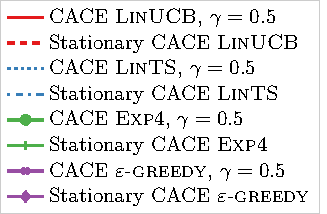
\includegraphics[width=0.85\linewidth]{sections/appendix/nips2020-bandits/images/attack_reward/simulations/legend.pdf}
        %\caption{Lorem ipsum}
    \end{minipage}\hfill
    \begin{minipage}{0.25\linewidth}
    \centering
    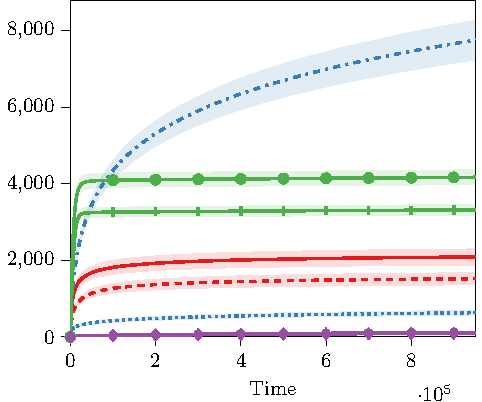
\includegraphics[width=0.95\linewidth]{sections/appendix/nips2020-bandits/images/attack_reward/simulations/cost_attack_reward_simulations.pdf}
    % \caption{Synthetic}
    \end{minipage}\hfill
    \begin{minipage}{0.25\linewidth}
    \centering
    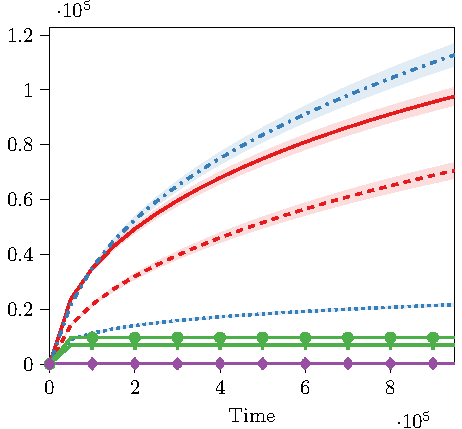
\includegraphics[width=0.85\linewidth]{sections/appendix/nips2020-bandits/images/attack_reward/jester/cost_attack_reward_jester.pdf}
    % \caption{Jester}
    \end{minipage}\hfill
    \begin{minipage}{0.25\linewidth}
    \centering
    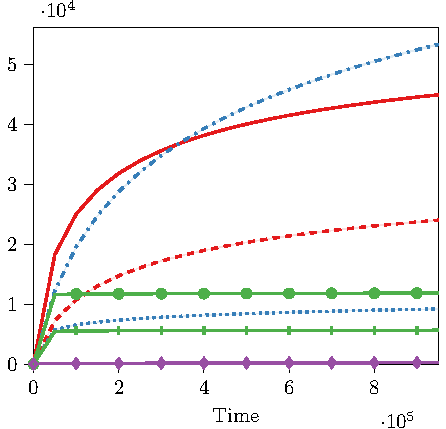
\includegraphics[width=0.85\linewidth]{sections/appendix/nips2020-bandits/images/attack_reward/movielens/cost_reward_attack_movielens.pdf}
    % \caption{MovieLens}
    \end{minipage}\\
    \begin{minipage}{0.25\linewidth}
        \centering
        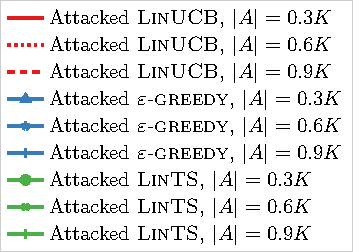
\includegraphics[width=0.85\linewidth]{sections/appendix/nips2020-bandits/images/regret_cost_attacks_context/simulations/legend.pdf}
        %\caption{Lorem ipsum}
    \end{minipage}\hfill
    \begin{minipage}{0.25\linewidth}
    \centering
    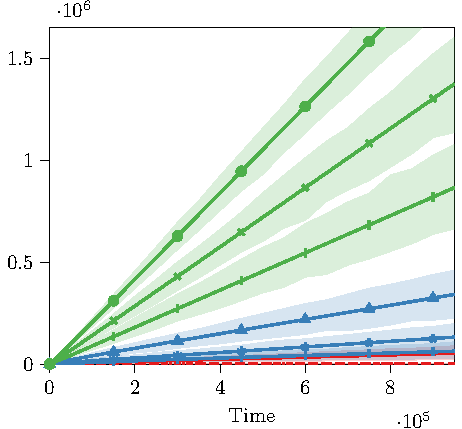
\includegraphics[width=0.95\linewidth]{sections/appendix/nips2020-bandits/images/regret_cost_attacks_context/simulations/cost_context_attack_simulations.pdf}
    % \caption{Synthetic}
    \end{minipage}\hfill
    \begin{minipage}{0.25\linewidth}
    \centering
    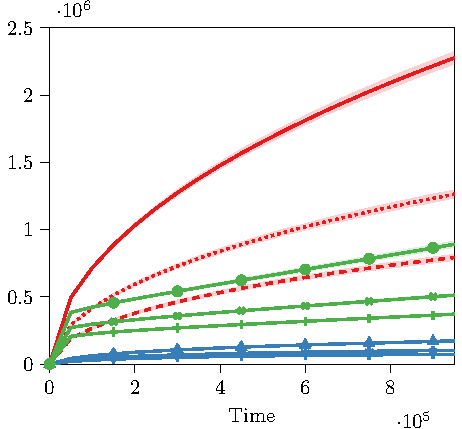
\includegraphics[width=0.85\linewidth]{sections/appendix/nips2020-bandits/images/regret_cost_attacks_context/jester/cost_context_attack_jester.pdf}
    % \caption{Jester}
    \end{minipage}\hfill
    \begin{minipage}{0.25\linewidth}
    \centering
    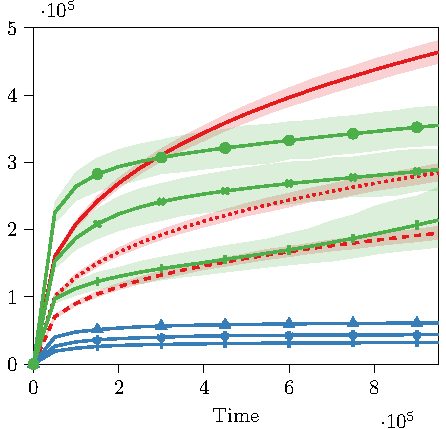
\includegraphics[width=0.85\linewidth]{sections/appendix/nips2020-bandits/images/regret_cost_attacks_context/movielens/cost_context_attack_movielens.pdf}
    % \caption{MovieLens}
    \end{minipage}
    \caption{Total cost of attacks on rewards for the synthetic (Left, $\gamma=0.22$), Jester (Center, $\gamma=0.5$) and MovieLens (Right, $\gamma=0.5$) environments. Bottom, total cost of ContextualConic attacks on the synthetic (Left), Jester (Center) and MovieLens (Right) environments.\vspace{-0.5cm}}%. The cumulative cost of the attacks is sublinear and most attacks occur during the first few iterations.}
\label{fig:costs_plot}
\end{figure}

% \begin{figure}[t]
% \centering
% \begin{tabular}{cccc}
% % Legend & Synthetic & Jester & MovieLens\\
% \includegraphics[width=.22\columnwidth]{images/costs_attacks_rewards_no_legend/legend_rewards_attacks.pdf}&
% \includegraphics[width=.22\columnwidth]{images/costs_attacks_rewards_no_legend/gen_synth_cost.pdf}& 
% \includegraphics[width=.22\columnwidth]{images/costs_attacks_rewards_no_legend/gen_jester_cost.pdf}& 
% \includegraphics[width=.22\columnwidth]{images/costs_attacks_rewards_no_legend/gen_movielens_cost.pdf}\\
% %  Legend & Synthetic & Jester & MovieLens\\
% \includegraphics[width=.22\columnwidth]{images/attacks_all_contexts_no_legend/legend_all_contexts.pdf}&
% \includegraphics[width=.22\columnwidth]{images/attacks_all_contexts_no_legend/gen_cost.pdf}&
% \includegraphics[width=.22\columnwidth]{images/attacks_all_contexts_no_legend/gen_jester_cost.pdf}&
% \includegraphics[width=.22\columnwidth]{images/attacks_all_contexts_no_legend/gen_movielens_cost.pdf}\\
% \vspace{-0.1in}


% \end{tabular}%\\
% 	%~\vspace*{-0.4cm}~\\
% \caption{On the left, total cost of the attacks on the rewards on the synthetic and dataset-based environments with $\gamma =0.5$ for Jester and MovieLens and $\gamma=0.22$ for the synthetic dataset. On the right, total cost of ContextualConic attacks on the synthetic and dataset-based environments.\vspace{-0.5cm}}%. The cumulative cost of the attacks is sublinear and most attacks occur during the first few iterations.}
% \label{fig:costs_plot}
% % \vspace{-0.1in}
% \end{figure}
% \begin{figure}[t]
% \centering
% \includegraphics[width=0.4\textwidth]{images/all_contexts_3_algs_jester/gen_jester_cost.pdf}
% \includegraphics[width=.4\textwidth]{images/all_contexts_3_alg_movielens/gen_movielens_cost.pdf}
% \caption{Total cost of ContextualConic attacks on dataset-based environments (Jester above, Movielens below).}%. The cumulative cost of the attacks is sublinear and most attacks occur during the first few iterations.}
% \label{fig:datasets_all_context}
% \end{figure}
\vspace{-0.2cm}
\subsection{Offline attacks on a Single Context}
\vspace{-0.02in}
 %We study the setting described in section \ref{sec:attack_one_context}, where the attacker can only modify a single context. 
 We now move to the setting described in Sec.~\ref{sec:attack_one_context} and test the same algorithms as in Sec.~\ref{subsec:exp_attack_all_context}. We run 40 simulations for each algorithm \changebr{and each attack type}. The target context $x^{\dagger}$ is chosen randomly and the target arm as the arm minimizing the expected reward for $x^{\dagger}$. %the performance of \linucb, \epsgreedy and \lints on a synthetic dataset and two datasets based on real data - Jester and MovieLens. The datasets are preprocessed in the same way as for the other experiments and we use the same parameters for all the algorithms. We run 40 simulations for each algorithm. 
 %In this setting, we choose a target context randomly and define the target arm as the arm minimizing the reward in this context. 
 The attacker is only able to modify the incoming context for the target context (which corresponds to the context of one user) and the incoming contexts are sampled uniformly from the set of all possible contexts (of size $100$). %. Although our attacks do not require it, we limit the number of possible contexts to $100$ in order to be able to observe significant differences between the attacked and unattacked algorithms.
%  \begin{table}[t]
% \begin{center}
% \begin{tabular}{lccc}
% \toprule
% {} & Synthetic &  Jester & MovieLens \\
% \midrule
% \linucb             &      $0.07\%$ &   $0.01\%$ &    $0.39\%$ \\
% \linucb Relaxed     &     $13.76\%$ &  $97.81\%$ &    $4.09\%$ \\
% \linucb Full        &     $88.30\%$ &  $99.98\%$ &   $99.99\%$ \\
% \epsgreedy         &      $0.01\%$ &   $0.00\%$ &    $0.03\%$ \\
% \epsgreedy Full &     $99.98\%$ &  $99.95\%$ &   $99.97\%$ \\
% \lints              &      $0.02\%$ &   $0.01\%$ &    $0.05\%$ \\
% \lints Relaxed      &     $18.21\%$ &  $80.48\%$ &    $5.56\%$ \\
% \bottomrule
% \end{tabular}
% \caption{Percentage of times  an algorithm pulled the target arm $a^{\dagger}$ when context $x^{\star}$ was drawn, averaged on 40 runs of 1M iterations. When applicable, the Relaxed version corresponds to solving a relaxed convex version of the problem while the Full attack corresponds to solving the exact optimization problem.
% \label{table:success_rates_one_ctx}
% \vspace{-0.3cm}
% }
% \end{center}
% \end{table}
 Table~\ref{table:success_rate} (Right) shows the percentage of success for \changebr{each attack}. We observe that the non-relaxed attacks on \epsgreedy and \linucb work well across all datasets. %is also very successful on datasets based on real data, and quite successful on synthetic datasets. 
 However, the relaxed attack %solving the problems with convex relaxations of the constraints 
 for \linucb and \lints are not as successful, on the synthetic dataset and MovieLens25M. 
 The Jester dataset seems to be particularly suited to this type of attacks because the true feature vectors are well separated from the convex hull formed by the feature vectors of the other arms: only $5$\% of Jester's feature vectors are within the convex hull of the others versus $8\%$ for MovieLens and $20\%$ for the synthetic dataset.
 %\todo{Can we find a better explanation? The current one doesn't explain why the success rate is better in the synthetic dataset than in MovieLens (probably because there are less arms)}
 As expected, the cost of the attacks is linear on all the datasets (see Figure \ref{fig:cost_attack_one_ctx} in App.~\ref{app:additional_fig_one_ctx}). The cost is also lower for the non-relaxed than for the relaxed version of the attack on \linucb. Unsurprisingly, the cost of the attacks on \lints is the highest %higher than for the other algorithms 
due to the need to guarantee that %the arm 
$a^{\dagger}$ will be chosen with high probability (95\% in our experiments).

% \subsection{Size of $A^\dagger$}
% \begin{figure}
%     \centering
%     \begin{minipage}{0.3\linewidth}
%         \centering
%         \includegraphics[width=\linewidth]{images/target_sets_simulations/attacks_norms_set_targets_all_context_linucb_sets_targets_simulations.pdf}
%         %\caption{Lorem ipsum}
%     \end{minipage}\hfill
%     \begin{minipage}{0.3\linewidth}
%     \centering
%     \includegraphics[width=\linewidth]{images/target_sets_jester/attacks_norms_allall_context_linucb_sets_targets_jester.pdf}
%     % \caption{Synthetic}
%     \end{minipage}\hfill
%     \begin{minipage}{0.3\linewidth}
%     \centering
%     \includegraphics[width=\linewidth]{images/target_sets_movielens/attacks_norms_all_context_linucb_sets_targets_movielens.pdf}
%     % \caption{Jester}
%     \end{minipage}\hfill\\
%         \begin{minipage}{0.3\linewidth}
%         \centering
%         \includegraphics[width=\linewidth]{images/target_sets_simulations/regret_all_context_linucb_sets_targets_simulations.pdf}
%         %\caption{Lorem ipsum}
%     \end{minipage}
%     \begin{minipage}{0.3\linewidth}
%     \centering
%     \includegraphics[width=\linewidth]{images/target_sets_jester/regret_all_context_linucb_sets_targets_jester.pdf}
%     % \caption{Synthetic}
%     \end{minipage}
%     \begin{minipage}{0.3\linewidth}
%     \centering
%     \includegraphics[width=\linewidth]{images/target_sets_movielens/regret_all_context_linucb_sets_targets_movielens.pdf}
%     % \caption{Jester}
    
%     % \caption{MovieLens}
%     \end{minipage}
%     \caption{From left to right, effect of the size of $A^\dagger$ on the regret and the norm of the attacks.}
% \label{fig:costs_plot}
% \end{figure}
% \begin{figure}[h]
%     \centering
%     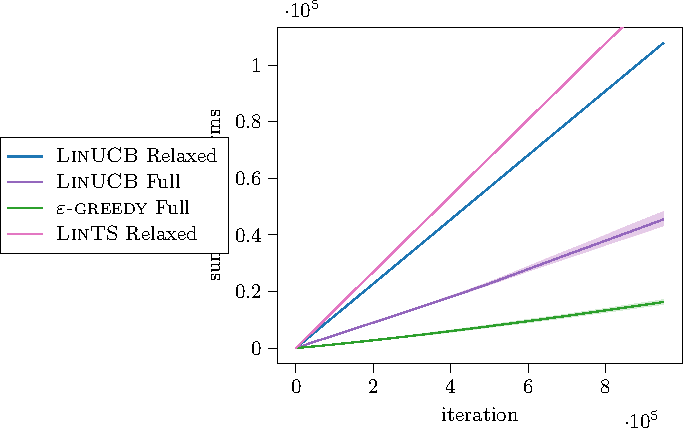
\includegraphics[width=0.45\textwidth]{images/one_context_3_alg_sim/attacks_norms_allone_context_3_alg_sim_remade.pdf}
%     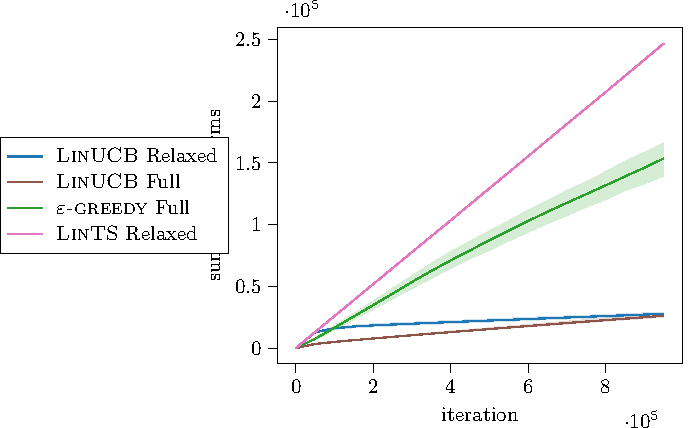
\includegraphics[width=0.45\textwidth]{images/one_context_3_alg_jester/attacks_norms_allone_context_3_alg_jester_remade.pdf}
%     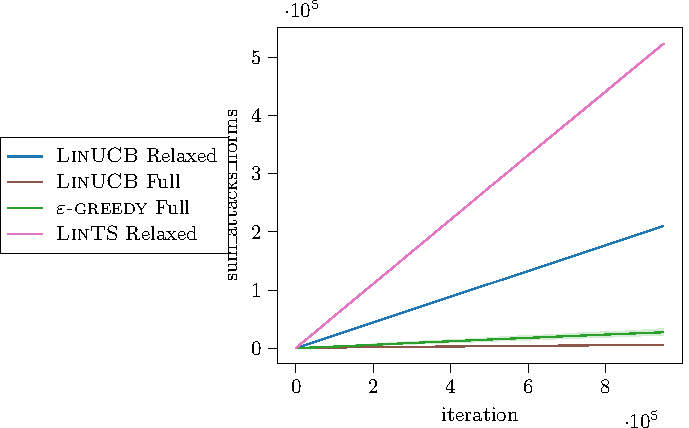
\includegraphics[width=0.45\textwidth]{images/one_context_3_alg_movielens/attacks_norms_allone_context_3_alg_movielens_remade.pdf}
%     \caption{Total cost of the attacks for the attacks one one context on our synthetic dataset, Jester and MovieLens. As expected, the total cost is linear.}
%     \label{fig:cost_attack_one_ctx}
% \end{figure}
% \include{images/long_term_attacks_graphs/attacks_norms_jester_not_all_context.tex}
% \begin{figure}[H]
% \includegraphics[width=.4\textwidth]{images/all_contexts_3_algs_jester/regret_all_contexts_3_alg_jester.png}
% \includegraphics[width=.4\textwidth]{images/all_contexts_3_algs_jester/attacks_norms_all_contexts_3_alg_jester.png}
% \includegraphics[width=.4\textwidth]{images/all_contexts_3_algs_jester/ratio_success_all_contexts_3_alg_jester.png}
% \includegraphics[width=.4\textwidth]{images/all_contexts_3_algs_jester/time_target_arm_chosen_all_contexts_3_alg_jester.png}
%   \caption{Jester experiment: from left to right, the regret, sum of the norms of the attacks, and percentage of successful attacks for each time step t for experiments conducted on the jester dataset. In blue, the attack described in section \ref{sec:attack_all_context}. In green, a version where attacks can only be performed on 20\% of the incoming contexts and the norm of the attack is multiplied by 5 to compensate. The regret for the attacked algorithms (in blue and green) is linear and the ratio of successful attacks quickly jumps close to 1. The cost of the attacks is only logarithmic (middle graph). The cost of the attacks is slightly smaller when their norms is greater (for the green curve). 95\% confidence intervals are represented on the curves, although they are often not visible. We removed the graphs of the attack norm for attacked \lints since they were linear and flattened the rest of the curves.\label{fig:jester}}
% \end{figure}
% \begin{figure}[H]
% \includegraphics[width=.4\textwidth]{images/all_contexts_3_alg_movielens/regret_all_context_3_alg_movielens.pdf}
% \includegraphics[width=.4\textwidth]{images/all_contexts_3_alg_movielens/attacks_norms_allall_context_3_alg_movielens.pdf}
% \includegraphics[width=.4\textwidth]{images/all_contexts_3_alg_movielens/ratio_success_all_context_3_alg_movielens.pdf}
% \includegraphics[width=.4\textwidth]{images/all_contexts_3_alg_movielens/a_star_chosenall_context_3_alg_movielens.pdf}
%   \caption{MovieLens experiment: from left to right, the regret, sum of the norms of the attacks, and percentage of successful attacks for each time step t for experiments conducted on the movielens dataset.\label{fig:movielens}}
% \end{figure}
% \begin{figure}[H]
%     \includegraphics[width=.4\textwidth]{images/all_context_3_alg_sim/regret_all_contexts_3_alg_sim.png}
%     \includegraphics[width=.4\textwidth]{images/all_context_3_alg_sim/attacks_norms_all_contexts_3_alg_sim.png}
%     \includegraphics[width=.4\textwidth]{images/all_context_3_alg_sim/ratio_success_all_contexts_3_alg_sim.png}
%         \includegraphics[width=.4\textwidth]{images/all_context_3_alg_sim/time_target_arm_chosen_all_contexts_3_alg_sim.png}
%   \caption{Experiments on synthetic dataset: from left to right, the regret, sum of the norms of the attacks, and percentage of successful attacks for each time step t for experiments conducted on the movielens dataset.\label{fig:simulations}}
%   \end{figure}
%   \begin{figure}[t]
%     % \includegraphics[width=.4\textwidth]{images/one_context_3_alg_sim/regret_one_context_3_alg_sim.pdf}
%     \includegraphics[width=.4\textwidth]{images/one_context_3_alg_sim/attacks_norms_allone_context_3_alg_sim.pdf}
%     \includegraphics[width=.4\textwidth]{images/one_context_3_alg_sim/a_star_chosenone_context_3_alg_sim.pdf}
%     % \includegraphics[width=.4\textwidth]{images/one_context_3_alg_sim/a_star_chosenone_context_3_alg_sim.pdf}
%         \includegraphics[width=.4\textwidth]{images/one_context_3_alg_sim/ratio_one_ctx_one_context_3_alg_sim.pdf}
%   \caption{Experiments on synthetic dataset for attacks one one context. We notice that epsilon greedy is relatively easier to attack, especially at the beginning (the ratio of successful attacks is higher faster) and the cost of the attacks is also comparatively lower. The attack cost is similar for \linucb and \lints but the attacks on \linucb are successful much more often. \label{fig:sim_one_ctx}}
%   \end{figure}
%     \begin{figure}[t]
%     \includegraphics[width=.4\textwidth]{images/one_context_3_alg_movielens/regret_one_context_3_alg_movielens.pdf}
%     \includegraphics[width=.4\textwidth]{images/one_context_3_alg_movielens/attacks_norms_allone_context_3_alg_movielens.pdf}
%     \includegraphics[width=.4\textwidth]{images/one_context_3_alg_movielens/a_star_chosenone_context_3_alg_movielens.pdf}
%     % \includegraphics[width=.4\textwidth]{images/one_context_3_alg_sim/a_star_chosenone_context_3_alg_sim.pdf}
%         \includegraphics[width=.4\textwidth]{images/one_context_3_alg_movielens/ratio_one_ctx_one_context_3_alg_movielens.pdf}
%   \caption{Experiments on movielens dataset for attacks one one context. The short-term attacks are successful for epsilon-greedy and when solving the non-relaxed version of the problem for \linucb (the success rate is close to 100\%). However, it fails most of the time for Linear Thomson Sampling and when solving the relaxed problem with \linucb: while the number of times the arm $a^{\dagger}$ is pulled in context $a^{\dagger}$ is way above that of the unattacked version, the success rate is still below 10\%. \label{fig:movielens_one_ctx}}  
%   \end{figure}
%     \begin{figure}[t]
%     \includegraphics[width=.4\textwidth]{images/one_context_3_alg_jester/regret_one_context_3_alg_jester.pdf}
%     \includegraphics[width=.4\textwidth]{images/one_context_3_alg_jester/attacks_norms_allone_context_3_alg_jester.pdf}
%     % \includegraphics[width=.4\textwidth]{images/one_context_3_alg_movielens/a_star_chosenone_context_3_alg_sim_movielens.pdf}
%     % \includegraphics[width=.4\textwidth]{images/one_context_3_alg_sim/a_star_chosenone_context_3_alg_sim.pdf}
%     \includegraphics[width=.4\textwidth]{images/one_context_3_alg_jester/ratio_one_ctx_one_context_3_alg_jester.pdf}
%   \caption{Experiments on jester dataset for attacks one one context. On the jester dataset, all the types of attacks are reasonably successful. As for movielens (Fig. \ref{fig:movielens_one_ctx}), the attacked we obtained by solving the unrelaxed problems for epsilon-greedy and \linucb are almost always successful. Here, the relaxed attacks are also successful more than 75\% of the time for both Linear Thompson Sampling and \linucb. \label{fig:jester_one_ctx}}
%   \end{figure}
%      \begin{figure}[t]
%     \includegraphics[width=.4\textwidth]{images/one_context_3_alg_sim/regret_one_context_3_alg_sim.pdf}
%     \includegraphics[width=.4\textwidth]{images/one_context_3_alg_sim/attacks_norms_allone_context_3_alg_sim.pdf}
%     \includegraphics[width=.4\textwidth]{images/one_context_3_alg_sim/a_star_chosenone_context_3_alg_sim.pdf}
%     % \includegraphics[width=.4\textwidth]{images/one_context_3_alg_sim/a_star_chosenone_context_3_alg_sim.pdf}
%         \includegraphics[width=.4\textwidth]{images/one_context_3_alg_sim/ratio_one_ctx_one_context_3_alg_sim.pdf}
%   \caption{Experiments on a simulated dataset for one context \label{fig:sim_one_ctx}}  
%   \end{figure}
%       \begin{figure}[t]
%     \includegraphics[width=.4\textwidth]{images/rewards_attacks_jester/avg_regret.png}
%     \includegraphics[width=.4\textwidth]{images/rewards_attacks_jester/avg_cost.png}
%     \includegraphics[width=.4\textwidth]{images/rewards_attacks_jester/avg_draws.png}
%   \caption{Reward attacks jester \label{fig:jester_reward_attacks}}
%   \end{figure}
%         \begin{figure}[t]
%     \includegraphics[width=.4\textwidth]{images/rewards_attacks_movielens/avg_regret.png}
%     \includegraphics[width=.4\textwidth]{images/rewards_attacks_movielens/avg_cost.png}
%     % \includegraphics[width=.4\textwidth]{images/one_context_3_alg_movielens/a_star_chosenone_context_3_alg_sim_movielens.pdf}
%     % \includegraphics[width=.4\textwidth]{images/one_context_3_alg_sim/a_star_chosenone_context_3_alg_sim.pdf}
%     \includegraphics[width=.4\textwidth]{images/rewards_attacks_movielens/avg_draws.png}
%   \caption{Reward attacks movielens \label{fig:movielens_reward_attacks}}
%   \end{figure}
%       \begin{figure}[t]
%     \includegraphics[width=.4\textwidth]{images/rewards_attacks_simulations/avg_regret.png}
%     \includegraphics[width=.4\textwidth]{images/rewards_attacks_simulations/avg_cost.png}
%     % \includegraphics[width=.4\textwidth]{images/one_context_3_alg_movielens/a_star_chosenone_context_3_alg_sim_movielens.pdf}
%     % \includegraphics[width=.4\textwidth]{images/one_context_3_alg_sim/a_star_chosenone_context_3_alg_sim.pdf}
%     \includegraphics[width=.4\textwidth]{images/rewards_attacks_simulations/avg_draws.png}
%   \caption{Reward attacks simulations \label{fig:sim_reward_attacks}}
%   \end{figure}
